\documentclass[]{article}
\usepackage[ngerman]{babel}
\usepackage[utf8]{inputenc}
\usepackage{amssymb}
\usepackage{amsmath}
\usepackage[all]{xy}
\usepackage{graphics,color} 
\usepackage{graphicx}
\usepackage{float}
\usepackage{amsthm}
\newtheorem{Definition}{Definition}
\newtheorem{Beispiel}{Beispiel}
\newtheorem{Satz}{Satz}
\newtheorem{Bemerkung}{Bemerkung}

\newtheorem{Algorithmus}{Algorithmus}

\begin{document}

\title{Einführung in die Computergrafik}
\author{Johannes Riesterer}
\date{\today}
\maketitle
\newpage 
\begin{center}
\large
 \copyright Johannes Riesterer \\
Vervielfältigung nur mit ausdrücklicher Erlaubnis des Autors
\end{center}

\newpage

\section*{Vorwort}


\tableofcontents
\newpage

\section{Mathematische Werkzeuge}

\subsection{Lineare Algebra}
\subsubsection{Vektoren und Matrizen}
Wir wollen zunächst  den Vektorraum $\mathbb{R}^n$ einführen. Hierbei ist $n$ eigentlich immer $2,3$ oder $4$.
Zunächst ist der $\mathbb{R}^n$  eine Menge, nämlich die Menge der $n$-dimensionalen Vektoren 
\begin{align*}
\mathbb{R}^n : = \Biggl \{
\begin{pmatrix}
x_1 \\ x_2 \\ \vdots \\ x_n
\end{pmatrix} \Bigg | \; x_1, x_2, \hdots ,x_n \in \mathbb{R}
 \Biggr \}  \; .
\end{align*}
Auf dieser Menge der Vektoren definiert man die Addition
\begin{align*}
+ : \mathbb{R}^n \times  \mathbb{R}^n   & \to \mathbb{R}^n \\
\begin{pmatrix}
x_1 \\ x_2 \\ \vdots \\ x_n
\end{pmatrix}  +  
\begin{pmatrix}
y_1 \\ y_2 \\ \vdots \\ y_n
\end{pmatrix} 
&  :=  \begin{pmatrix}
x_1 + y_1 \\ x_2  + y_2 \\ \vdots \\ x_n + y_n
\end{pmatrix} 
\end{align*}

und die sogenannte Skalarmultiplikation 
\begin{align*}
\cdot : \mathbb{R} \times  \mathbb{R}^n   & \to \mathbb{R}^n \\
\lambda \cdot \begin{pmatrix}
x_1 \\ x_2 \\ \vdots \\ x_n
\end{pmatrix}  
&  :=  \begin{pmatrix}
\lambda  \cdot x_1  \\  \lambda \cdot x_2 \\ \vdots \\  \lambda \cdot x_n 
\end{pmatrix} \; . 
\end{align*}
Das Element $\lambda  \in \mathbb{R}$ nennt man auch Skalar.
\begin{Definition}
Der Vektorraum $\mathbb{R}^n$ ist das Tripel 
$(\mathbb{R}^n, + , \cdot )$.
\end{Definition}

\begin{Beispiel}
\begin{align*}
\begin{pmatrix}
1 \\ 2  \\  3
\end{pmatrix}  +  
\begin{pmatrix}
3 \\ 2  \\ 1
\end{pmatrix} 
=  \begin{pmatrix}
4 \\ 4  \\ 4
\end{pmatrix} 
\end{align*}

\begin{align*}
\begin{pmatrix}
 1 \\  1 
\end{pmatrix}  +  
\begin{pmatrix}
-1  \\  -1 
\end{pmatrix} 
=  \begin{pmatrix}
0  \\  0 
\end{pmatrix}  
\end{align*}

\begin{align*}
\begin{pmatrix}
1 \\ -1  \\  -\frac{1}{2}  \\ 2 
\end{pmatrix}  +  
\begin{pmatrix}
0  \\  0 \\  0 \\ 0
\end{pmatrix} 
=  \begin{pmatrix}
1 \\ -1  \\  -\frac{1}{2}  \\ 2 
\end{pmatrix} 
\end{align*}

\begin{align*}
-1 \cdot
\begin{pmatrix}
1 \\ 1  \\  1 
\end{pmatrix}  
=  \begin{pmatrix}
-1   \\ -  1    \\  -1  
\end{pmatrix} 
\end{align*}

 
\begin{align*}
\pi \cdot
\begin{pmatrix}
1 \\ 2  \\  3 \\ 4
\end{pmatrix}  
=  \begin{pmatrix}
\pi   \\ 2  \pi  \\  3 \pi \\  4  \pi
\end{pmatrix} 
\end{align*}

\begin{Bemerkung}
Für alle Skalare $\lambda, \mu \in \mathbb{R}$ und Vektoren $u,v \in  \mathbb{R}^n$ gelten die  Rechenregeln
\begin{align*}
\lambda \cdot (u +v) = \lambda \cdot u + \lambda \cdot v \\
(\lambda + \mu)  \cdot u  = \lambda  \cdot u + \mu  \cdot u \; .
\end{align*}
\end{Bemerkung}

\begin{Definition}
Für ein $u,v \in  \mathbb{R}^n$ sind die folgenden Kurz-Notationen üblich
\begin{align*}
-u :=  -1 \cdot u \\
u -v := u + (-v) := u + (-1 \cdot u) 
\end{align*}  
\end{Definition}
\end{Beispiel}

\begin{Definition}
Eine $n \times m$ Matrix ist ein Objekt der Form
\begin{align*}
(a_{ij})_{ij} := \begin{pmatrix}
a_{1,1} &  a_{1,2} & a_{1,3} & \cdots & a_{1,m}   \\  
a_{2,1} &  a_{2,2} & a_{2,3} & \cdots & a_{2,m} \\  
 \vdots &  \vdots &\vdots & \vdots & \vdots & \\ 
a_{i,1} &  a_{i,2} & a_{i,3} & \cdots & a_{i,m} \\
 \vdots &  \vdots &\vdots & \vdots & \vdots & \\ 
a_{n,1} &  a_{n,2} & a_{n,3} & \cdots & a_{n,m}  
\end{pmatrix}  
\end{align*} 
mit $a_{i,j} \in \mathbb{R}$ für alle $i = 1, \hdots, n$ und $j = 1, \hdots m$.
\end{Definition}


\begin{Bemerkung}
Ein Vektor der dimension $n$ ist eine $n \times 1$-Matrix.
\end{Bemerkung}
\begin{Definition}
Ist $A = (a_{ij})_{ij}$ eine $n \times m$ und $B = (b_{kl})_{kl}$ eine $m \times p$ Matrix so
ist das Matrizenprodukt definiert als die $n \times p$ Matrix
\begin{align*}
A \cdot B := \Biggl( \sum_{j=1}^{m}a_{ij} \cdot b_{jl} \Biggr)_{il} \; .
\end{align*}
Sind $A$ und $B$  zwei $n \times m$-Matrizen so ist ihre Summer definiert durch 
\begin{align*}
A + B := \biggl( a_{ij} + b_{ij} \biggr)_{ij} \;.
\end{align*}
Für ein $\lambda \in \mathbb{R}$ definieren wir die Skalarmultiplikation
\begin{align*}
\lambda \cdot A := \biggl( \lambda \cdot a_{ij} \biggr)_{ij} \;.
\end{align*}
\end{Definition}


\begin{Definition}
Die $n$-dimensionale Einheitsmatrix ist definiert durch
\begin{align*}
I_n : = \begin{pmatrix}
1 & 0 & 0 & \cdots & 0 & 0 \\
0 & 1 & 0 & \cdots & 0 & 0 \\
\vdots &  & \ddots &  & \vdots & \vdots \\
\vdots &  &  &  \ddots & 0 & 0 \\
0 & 0 & 0 & \cdots & 1 & 0 \\
0 & 0 & 0 & \cdots & 0 & 1
\end{pmatrix} \; .
\end{align*}
\end{Definition}

\begin{Bemerkung}
Sind $A$ und $B$ beides $n\times n$-Matrizen, so ist im Allgemeinen
\begin{align*}
A \cdot B \neq B \cdot A \; .
\end{align*}
Für die $n$-te Einheitsmatrix $I_n$ gilt jedoch immer
\begin{align*}
A \cdot I_n =  I_n \cdot A  = A \; .
\end{align*}
\end{Bemerkung}


\begin{Definition}
Für eine $2 \times 2$-Matrix definieren wir die Determinante
\begin{align*}
\det : M^{n \times n}  & \to \mathbb{R} \\
\det \biggl ( 
\begin{pmatrix}
a & b \\ c & d
\end{pmatrix}
 \biggr)  & := ad - bc
\end{align*}
\end{Definition}


\begin{Satz}
Für eine $n \times n$ Matrix $A = (a_{ij})_{ij}$ definieren wir die Determinante durch die Rekursionsformel
\begin{align*}
det (A) = \sum_{j=1}^n  (-1)^{i+j} a_{ij} det (A_{ij})
\end{align*}
und $det (a) = a$ für eine $1 \times 1$-Matrix $a$.
wobei $A_{ij}$ die Matrix ist, die aus $A$ durch Streichen der $i$-ten Zeile und der $j$-ten Spalte entsteht.
Diese Definition ist unabhängig von der Wahl von $i$. (Entwickeln nach der $i-ten Zeile$).
\end{Satz}

\begin{Satz}
Für alle $n \times n$-Matrizen $A,B$ gilt
\begin{align*}
\det(A \cdot B) = \det(A) \cdot \det(B)
\end{align*} \; .
\end{Satz}
\begin{Satz}
Sei $A$ eine $n \times n$ Matrix. Dann existiert genau dann eine Matrix $A^{-1}$ mit
\begin{align*}
A \cdot A^{-1}  = A^{-1} \cdot A  = I_n \; ,
\end{align*}
wenn $\det(A) \neq 0$. $A^{-1}$ ist eindeutig bestimmt.
\end{Satz}
\begin{Bemerkung}
Ist $v$ ein $n$-dimensionaler Vektor und $A$ eine $m\times n$-Matrix, so ist 
$A \cdot v$ ein $m$-dimensionaler Vektor.
\end{Bemerkung}

\begin{Definition}
Ist $A := (a_{ij}))_{ij}$ eine $n \times m$-Matrix, so heißt die $m \times n$-Matrix 
$A ^t := (a_{ji}))_{ij}$ die transponierte Matrix. 
\end{Definition}


\begin{Definition}
Ist insbesondere $v= \begin{pmatrix}
x_1 \\ \vdots \\ x_k
\end{pmatrix}
$ ein $k$-dimensionaler Vektor, so heisst
$v^t= \begin{pmatrix}
x_1 & \cdots & x_n
\end{pmatrix}$ der transponierte Vektor, welcher auch eine $1\times n$-Matrix ist.
\end{Definition}

\begin{Satz}
Für alle $n \times m$-Matrizen $A$ und $m$-dimensionale Vektoren $u,v$ gilt
\begin{align*}
A \cdot (\lambda \cdot u + \mu \cdot v) = \lambda \cdot A \cdot u +  \mu  \cdot A \cdot v \; .
\end{align*}
\end{Satz}

\begin{Definition}
Vektoren $v_1, \hdots ,v_k \in \mathbb{R}^n$ heißen linear unabhängig, falls für $\lambda_i \in \mathbb{R}, \; i=1, \hdots ,k $ mit
\begin{align*}
\sum_{i= 1}^k \lambda_i \cdot v_i = 0
\end{align*} 
stets $\lambda_i = 0$ folgt für alle $i = 1, \hdots, k$. 
\end{Definition}

\begin{Satz}
Die Vektoren $v_1, \hdots ,v_k \in \mathbb{R}^n$ sind genau dann linear abhängig, wenn man 
mit Hilfe des Gaussalgorithmus in der Matrix 
\begin{align*}
\begin{pmatrix}
v_1^t \\   \text{---} \\ \vdots \\  \text{---} \\ v_k^t
\end{pmatrix}
\end{align*}
eine Nullzeile erzeugen kann.
\end{Satz}

\begin{Bemerkung}
Für $k>n$ sind $v_1, \hdots ,v_k \in \mathbb{R}^n$ stets linear abhängig.
\end{Bemerkung}

\begin{Definition}
Für Vektoren $v_1, \hdots , v_k \in \mathbb{R}^n$ heißt die Menge
\begin{align*}
span(v_1, \hdots v_k) : = \biggl\{ \sum_{i=1}^k \lambda_i \cdot v_i \; | \; \lambda_i \in \mathbb{R}  \biggr\} \subseteq \mathbb{R}^n
\end{align*}
der von ihnen aufgespannte lineare Unterraum. Diese Definition ist offensichtlich unabhängig von der Reihenfolge. 
Eine Menge von Vektoren $\{ w_1, \hdots , w_l \}$ heißt Basis von
$span(v_1, \hdots v_k)$, falls $w_1, \hdots , w_l$ linear unabhängig sind und
$span(w_1, \hdots w_l) = span(v_1, \hdots v_k)$ gilt. $l$ heißt dann auch die Dimension von $span(v_1, \hdots v_k)$. 
\end{Definition}


\begin{Satz}
Ist $B:= \{ b_1, \hdots , b_n \}$ eine Menge linear unabhängiger $n$-dimensionaler Vektoren, so ist
\begin{align*}
span(b_1, \hdots ,b_n) = \mathbb{R}^n \; .
\end{align*}
Wir nennen dann die \emph{geordnete} Menge $B$ eine Basis des $\mathbb{R}^n$. 
\end{Satz}


\begin{Definition}
Wir bezeichnen die Basis $E:= \{ e_1, \hdots , e_n \}$ des $\mathbb{R}^n$ mit 
\begin{align*}
e_i : = \begin{pmatrix}
0 \\ \vdots \\ 0 \\ 1  \\ 0 \\ \vdots \\ 0
\end{pmatrix}
\begin{matrix}
 \\   \\  \leftarrow \text{i-te Stelle}  \\ \\  \\ 
\end{matrix}
\end{align*}
als Standardbasis des $\mathbb{R}^n$.
\end{Definition}

\begin{Definition}
Sei $B:= \{ b_1, \hdots , b_n \}$ eine Basis des $\mathbb{R}^n$ und $v \in \mathbb{R}^n$. Dann gibt es nach dem letzten Satz Skalare $\lambda_1, \hdots , \lambda_n \in \mathbb{R}$, so dass sich $v$ als Linearkombination 
\begin{align*}
v = \sum_{i=1}^n \lambda_i \cdot b_i 
\end{align*}
ausdrücken lässt. Schreibt man diese $\lambda_i$ wieder in einen Vektor, so erhalten wir eine Abbildung
\begin{align*}
\theta_B : \mathbb{R}^n & \to \mathbb{R}^n \\
\begin{pmatrix}
v_1 \\ \vdots \\ v_n
\end{pmatrix}
& \mapsto 
\begin{pmatrix}
\lambda_1 \\ \vdots \\ \lambda_n
\end{pmatrix} \; .
\end{align*}
Man nennt $\theta_B(v)$ die Darstellung von $v$ zur Basis $B$.
\end{Definition}

\begin{Bemerkung}
Für die Standardbasis $E$ des $\mathbb{R}^n$ ist $\theta_E(v) = v$ für alle $v \in \mathbb{R}^n$, also $\theta_S = \text{id}$.
\end{Bemerkung}

\begin{Definition}
Sei $B:= \{ b_1, \hdots , b_n \}$ eine Basis des $\mathbb{R}^n$ und $v \in \mathbb{R}^n$. Dann definieren wir  
\begin{align*}
M_B  = \biggl ( b_1 \; \bigg | \;  b_2 \; \bigg | \;  \cdots  \; \bigg | \;  b_n \biggr )^{-1}   \;.
\end{align*}
\end{Definition}


\begin{Satz}
Sei $B:= \{ b_1, \hdots , b_n \}$ eine Basis des $\mathbb{R}^n$ und $v \in \mathbb{R}^n$. Dann ist 
\begin{align*}
\theta_B (v) = M_B \cdot v   
\end{align*}
\end{Satz}



\begin{Definition}
Seien $B:= \{ b_1, \hdots , b_n \}$ und $B':= \{ b'_1, \hdots , b'_n \}$ zwei Basen des $\mathbb{R}^n$.
Dann heißt $M_{B}^{B'} : = M_{B'}  \cdot M_{B}^{-1} $ die Basiswechselmatrix von $B$ nach $B'$. Wir haben also folgende Situation:

\begin{align*}
\xymatrix{
\mathbb{R}^n  \ar[d]^{I_n} &  & \ar[ll]^{M_B^{-1}} \mathbb{R}^n \ar[d]^{M_{B}^{B'}} \\
\mathbb{R}^n  \ar[rr]^{M_{B'}} & &  \mathbb{R}^n
}
\end{align*}
\end{Definition}

\begin{Definition}
Die Abbildung 
\begin{align*}
< \cdot \; , \;  \cdot > : \mathbb{R}^n \times \mathbb{R}^n & \to \mathbb{R} \\
\Biggl < \begin{pmatrix}
x_1 \\ \vdots \\ x_n
\end{pmatrix},  \begin{pmatrix}
y_1 \\ \vdots \\ y_n
\end{pmatrix}  \Biggr> & := \begin{pmatrix}
x_1 \\ \vdots \\ x_n
\end{pmatrix}^t \cdot \begin{pmatrix}
y_1 \\ \vdots \\ y_n  
\end{pmatrix}  =
\begin{pmatrix}
x_1 & \cdots & x_n
\end{pmatrix} \cdot \begin{pmatrix}
y_1 \\ \vdots \\ y_n  
\end{pmatrix} = \sum_{i=1}^n  x_i \cdot y_i
\end{align*}  
heißt Skalarprodukt.
\end{Definition}



\begin{Satz}
Für alle $u,v,w,l \in \mathbb{R}^n$ und $\lambda, \mu, \tau, \nu \mathbb{R}$ gilt
\begin{align*}
<\lambda u + \mu v, \tau w> = \lambda \tau<u,w> + \mu \tau <v,w> \\
<\lambda u , \tau w + \nu l> = \lambda \tau<u,w> + \lambda \nu <u,l>
\end{align*}
\end{Satz}
\begin{Definition}
Die Abbildung 
\begin{align*}
|| \cdot || &: \mathbb{R}^n  \to \mathbb{R} \\
||v||  &:= \sqrt{<v,v>} 
\end{align*}  
heißt Norm.
\end{Definition}

\begin{Definition}
Zwei vom Nullvektor verschiedene Vektoren $u,v \in \mathbb{R}^n$ heißen orthogonal, falls $<u,v> = 0$ ist. 
Man sagt auch sie stehen senkrecht aufeinander und benutz auch die Bezeichnung $u \perp v$. 
\end{Definition}

\begin{Definition}
Sind $u = $ und $v$ zwei $3$-dimensionale Vektoren, dann heißt der Vektor
\begin{align*}
u \times v := 
\end{align*}
 das Kreuzprodukt von $u$ und $v$.
\end{Definition}

\begin{Bemerkung}
Für $u , v \in \mathbb{R}^n$ gilt
\begin{align*}
<u \times v, u> = <u \times v, v> = 0 \; . 
\end{align*}
Das Kreuzprodukt steht also senkrecht auf $u$ und auf $v$.
\end{Bemerkung}

\begin{Definition}
Ein Vektor $v \in \mathbb{R}$ heißt normal, falls $||v|| = 1$ ist.
Ist $w \in \mathbb{R}^n$ ein beliebiger Vektor, so heißt $\frac{1}{||w||} w$ die Normalisierung von $w$.
\end{Definition}

\begin{Definition}
Eine Basis  $B:= \{ b_1, \hdots , b_n \}$ heißt Orthonormalbasis (kurz ONB), falls 
\begin{align*}
<b_i, b_j> = \begin{cases}  1 \; \text{falls }  i = j  \\ 0 \; \text{sonst}\end{cases}
\end{align*}
gilt. Insbesondere sind alle $b_i$ normal.
\end{Definition}

\begin{Algorithmus}
Seien  $v_1, \hdots v_n$ linear unabhängige Vektoren.  Dann lässt sich daraus durch folgenden Algorithmus 
eine ONB generieren: 
\begin {align*}
b_i ' & := v_i - \sum_{j=1}^{i-1} <v_i, b_j> b_j \\
b_i  & :=  \frac{1}{||b_i||} b_i'
\end{align*}
und Rekursionsanfang $b_1' = v_1$.
\end{Algorithmus}


Im $\mathbb{R}^3$ gibt es eine besonders einfache Methode aus zwei Vektoren einen Vektor zu generieren, der auf den Ausgangs-Vektoren
senkrecht steht.
\begin{Definition}
Für $u = \begin{pmatrix} u_1 \\ u_2 \\ u_3 \end{pmatrix}$ und $v= \begin{pmatrix} v_1 \\ v_2 \\ v_3 \end{pmatrix}$ heißt
\begin{align*}
u \times v :=  \begin{pmatrix} u_2 v_3 - u_3v_2  \\ u_3 v_1 - u_1v_3 \\ u_1 v2 - u_2 v_1\end{pmatrix} 
\end{align*}
das Kreuzprodukt von $u$ und $v$.
\end{Definition}

\begin{Bemerkung}
Es gilt
\begin{itemize}
\item $<u \times v, u> =  <u \times v, v> = 0$ 
\item $u \times v = - (v \times u)$
\item $u \times v = 0$ genau dann, wenn $u$ und $v$ linear abhängig sind.
\end{itemize}
\end{Bemerkung}

\begin{Bemerkung}
Ist  $B:= \{ b_1, \hdots , b_n \}$  eine ONB, so gilt
\begin{align*}
M_{B}^{-1} = M_{B}^t
\end{align*}
\end{Bemerkung}

\begin{Definition}
Eine Matrix $O \in \mathbb{M}^{n \times n}$ heißt orthogonal, falls
$O^{-1} = O^t$ ist. 
\end{Definition}

\begin{Satz}
Eine Matrix $O \in \mathbb{M}^{n \times n}$ ist genau dann  orthogonal, falls
\begin{align*}
\det(O) \in  \{-1, 1 \} \; .
\end{align*}
Ist $\det(O) = 1$, so nennen wir $O$ eine Drehung und 
$SO(n) := \{ \}$ die Drehgruppe (oder auch spezielle orthogonale Gruppe).
\end{Satz}

\begin{Satz}
Sei $O \in \mathbb{M}^{n \times n}$ eine orthogonale Matrix, dann gilt für alles $v,w \in \mathbb{R}^n$
\begin{align*}
< O \cdot v \; , \;  O \cdot W > = <v \; , \; w>
\end{align*}
und somit insbesondere 
\begin{align*}
|| O \cdot v|| = ||v|| \; .
\end{align*}
\end{Satz}


\begin{Definition}
Eine $2 \times 2$-Drehmatrix ist eine Matrix der Form
\begin{align*}
\begin{pmatrix}
\cos(\varphi) & \pm \sin(\varphi) \\  \mp \sin(\varphi) & \cos(\varphi)
\end{pmatrix}
\end{align*}
für ein $\varphi \in [0, 2 \pi]$. 
\end{Definition}

\begin{Bemerkung}
Eine $2 \times 2$-Drehmatrix ist eine orthogonale Matrix.
\end{Bemerkung}



\begin{Definition}
Eine elementare $3 \times 3$-Drehmatrix ist eine Matrix der Form
\begin{align*}
\begin{pmatrix}
1 & 0 & 0 \\
0 & \cos(\varphi) & \pm \sin(\varphi) \\ 
 0 & \mp \sin(\varphi) & \cos(\varphi)
\end{pmatrix}, \;
\begin{pmatrix}
 \cos(\varphi) & 0 &  \pm \sin(\varphi) \\ 
0 & 1 & 0 \\ 
\mp \sin(\varphi) & 0& \cos(\varphi)
\end{pmatrix}, \;
\begin{pmatrix}
 \cos(\varphi) & \pm \sin(\varphi)  & 0\\ 
 \mp \sin(\varphi) & \cos(\varphi) & 0 \\
0 & 0 & 1 
\end{pmatrix}. 
\end{align*} 
für ein $\varphi \in [0, 2 \pi]$. 
\end{Definition}


\begin{Satz}
Jede Drehung  $O \in SO(3)$  lässt sich zerlegen in ein Produkt
\begin{align*}
O = 
\begin{pmatrix}
 \cos(\xi) &  \sin(\xi)  & 0\\ 
 - \sin(\xi) & \cos(\xi) & 0 \\
0 & 0 & 1 
\end{pmatrix} 
\cdot
\begin{pmatrix}
 \cos(\psi) & 0 &   \sin(\psi) \\ 
0 & 1 & 0 \\ 
- \sin(\psi) & 0& \cos(\psi)
\end{pmatrix}
\cdot \begin{pmatrix}
 \cos(\varphi) &  \sin(\varphi)  & 0\\ 
 - \sin(\varphi) & \cos(\varphi) & 0 \\
0 & 0 & 1 
\end{pmatrix} 
\end{align*} 
Die Winkel $\phi, \psi, \xi$ heißen  Eulerwinkel. 
\end{Satz}

\begin{Bemerkung}
Die  Zerlegung  $O \in SO(3)$  einer Drehung in obiges Produkt ist  nicht eindeutig.
Ein anschauliches Beispiel dafür liefert der sogenannte "Gimbal lock".
\end{Bemerkung}

\begin{figure}[H]
\centering
Kardansche Aufhängung und Gimbal lock\\
\includegraphics[scale=0.7]{images/gimbalLock.jpg}
\end{figure}

\begin{Bemerkung}
Man kann bei der Produktzerlegung auch andere elementare Drehmatratzen (elementare Drehachsen)  wählen, wobei
eine spezielle Wahl  zu den in der Luft und Raumfahrt verwendeten "Roll, Nick, Gier" Winkeln führen.
\end{Bemerkung}

\begin{figure}[H]
\centering
Roll, Nick und Gier Winkel \
\includegraphics[scale=0.6]{images/pitch.png}
\end{figure}

\subsection{Affiner Raum und affine Abbildungen}
Der Affine Raum $\mathbb{A}^n$ ist ein Tupel
\begin{align*}
\bigl( \mathbb{R}^n, (\mathbb{R}^n, + , \cdot ) \bigr )
\end{align*}
zusammen mit den Abbildung 
\begin{align*}
\text{---} : \mathbb{R}^n \times \mathbb{R}^n  & \to (\mathbb{R}^n, + , \cdot ) \\
\overline{PQ} & := Q-P  
\end{align*}
und
\begin{align*}
+ : \mathbb{R}^n \times (\mathbb{R}^n, + , \cdot )   & \to  \mathbb{R}^n\\
\begin{pmatrix}
P_1 \\ \vdots \\ P_n
\end{pmatrix} + \begin{pmatrix}
v_1 \\ \vdots \\ v_n
\end{pmatrix} & := \begin{pmatrix}
P_1  + v_1 \\ \vdots \\ P_n + v_n 
\end{pmatrix}   \;.
\end{align*}
Die Elemente (Vektoren) aus $\mathbb{R}^n$ nennt man auch  Punkte in Abgrenzung zu den Vektoren aus $(\mathbb{R}^n, + , \cdot )$.  
Für Punkte $P,Q \in \mathbb{R}^n$ ist also $\overline{PQ}$ ein Vektor, auch Verbindungsvektor genannt.

\begin{Definition}
Ist $B:= \{b_1, \hdots , b_n \}$ eine Basis des Vektorraums  $(\mathbb{R}^n, + , \cdot )$ und $P \in \mathbb{A}$ ein Punkt, so nennen wir das Tupel
$(P, B)$ eine affine Basis. Für jeden Punkt $Q$ gibt es dann also Skalare $\lambda_1,\hdots ,\lambda_n$ mit 
\begin{align*}
Q = P + \sum_{i=1}^{n} \lambda_i \cdot b_i  \; .
\end{align*}
Der Punkt $\begin{pmatrix}  \lambda_1 \\  \vdots \\  \lambda_n \end{pmatrix}$ heißt die Darstellung von $Q$ bezüglich der affinen Basis $(P,B)$. 
\end{Definition}



\begin{Definition}
Abbildungen der Form
\begin{align*}
\phi &: \mathbb{A} \to \mathbb{A} \\
\phi(P) & := A \cdot P + t
\end{align*} 
mit $A \in M^{n \times n}$ und $t \in (\mathbb{R}^n, + , \cdot )$ heißen affine Abbildungen.
Insbesondere heißt eine affine Abbildung mit $A = I_n$ und $t \neq 0$ Translation.
\end{Definition}

\begin{Bemerkung}
Eine Affine Abbildung
\begin{align*}
\phi &: \mathbb{A}^n \to \mathbb{A}^n \\
\phi(P) & := A \cdot P + t
\end{align*} 
ist genau dann invertierter, falls $\det(A) \neq 0$ ist und die Inverse Abbildung ist dann
\begin{align*}
\phi^{-1} &: \mathbb{A} \to \mathbb{A} \\
\phi^{-1}(P) & := A^{-1} \cdot P - A^{-1} \cdot t \; .
\end{align*} 
\end{Bemerkung}


\begin{Definition}
Sind $(P,B:= \{b_1, \hdots , b_n \})$  und $(P',B':= \{b'_1, \hdots , b'_n \})$ zwei affine Basen  und definieren wir 
die Abbildung
\begin{align*}
\theta_{(P,B)} & :  \mathbb{A}^n \to \mathbb{A}^n \\
\theta_{(P,B)}(Q) & := M_B \cdot Q - M_B \cdot P \; ,
\end{align*}
so erhalten wir analog zu der Situation in Vektorräumen
\begin{align*}
\xymatrix{
\mathbb{A}^n  \ar[d]^{\text{id}} &  & \ar[ll]^{\theta_{(P,B)}^{-1}} \mathbb{A}^n \ar[d]^{\theta_{(P,B)}^{(P',B')}} \\
\mathbb{A}^n  \ar[rr]^{\theta_{(P',B')}} & &  \mathbb{A}^n
}
\end{align*}
mit $\theta_{(P,B)}^{(P',B')} (Q) :=   \theta_{(P',B')} \biggl ( \theta_{(P,B)}^{-1} (Q) \biggr)$.
\end{Definition}


\begin{Definition}
Der Abstand von  $P,Q \in \mathbb{A}$  ist definiert durch
\begin{align*}
d : \mathbb{A} \times \mathbb{A} \to \mathbb{R} \\
d(P,Q) := || \overline{PQ} || \; .
\end{align*}
\end{Definition}


\subsubsection{Homogene Koordinaten und Projektionen}

\begin{Definition}
Der projektive  Raum ist definiert als
\begin{align*}
\mathbb{P}^n := \mathbb{R}^{n+1} / \sim \\
v \sim w \Leftrightarrow v = \lambda w \text{ für ein } \lambda \neq 0 \in \mathbb{R} \; . 
\end{align*}
\end{Definition}

Wir haben die Abbildung
\begin{align*}
\mathbb{A}^n & \to \mathbb{P}^n \\
\begin{pmatrix} p_1 \\ p_2 \\ \vdots \\ p_n \end{pmatrix} & \mapsto \begin{pmatrix} p_1 \\ p_2 \\ \vdots \\ p_n  \\  1\end{pmatrix} 
\end{align*}
und nennen das Bild eines Punktes unter dieser Abbildung die homogenen Koordinaten.
Auf der Menge der homogenen Koordinaten haben wir die Umkehrabbildung
\begin{align*}
& \mathbb{P}^n - \Biggl \{ \begin{pmatrix} p_1 \\ p_2 \\ \vdots \\ p_n  \\  p_{n+1} \end{pmatrix} \Bigg | \; p_{n+1} \neq 0 \Biggr \}   \to \mathbb{A}^n \\
& \begin{pmatrix} p_1 \\ p_2 \\ \vdots \\ p_n  \\  p_{n+1} \end{pmatrix}   \mapsto \begin{pmatrix}  \frac{p_1}{ p_{n+1}} \\ \frac{p_2}{ p_{n+1}}  \\ \vdots \\ \frac{p_n}{ p_{n+1}}  \end{pmatrix}  \; .
\end{align*}


Die Matrizenmultiplikation
\begin{align*}
\mathbb{R}^{n+1} \to \mathbb{R}^{n+1} \\
v \mapsto A \cdot v
\end{align*}
setzt sich wegen der Eigenschaft $A \cdot (\lambda v) = \lambda A \cdot v$ zu einer Abbildung
\begin{align*}
\mathbb{P}^{n} \to \mathbb{P}^{n} \\
p \mapsto A \cdot p
\end{align*}
fort. Wir können damit und mit der Definition der Matrix-Vektor-Multiplikation eine affine Abbildung 
\begin{align*}
\phi : \mathbb{R}^{n} \to \mathbb{R}^{n} \\
\phi(v):=  A \cdot v + t
\end{align*}
in homogenen Koordinate ausdrücken durch eine Matrizenmultiplikation
\begin{align*}
\begin{pmatrix} v \\ 1\end{pmatrix} \mapsto \begin{pmatrix}  A  & t  \\ 0 &1\end{pmatrix} \cdot  \begin{pmatrix} v \\ 1\end{pmatrix}   \; .
\end{align*}

\begin{Definition}
Die Abbildung 
\begin{align*}
persp_{xy} : \mathbb{A}^3 \to \mathbb{A}^2 \\
\begin{pmatrix}  X \\ Y \\ Z\end{pmatrix}  \mapsto \begin{pmatrix}  \frac{X}{\frac{Z}{d} +1 } \\   \frac{X}{\frac{Z}{d} +1 } \end{pmatrix}
\end{align*}
die Zentralprojektion auf die $X-Y$-Ebene mit Augendistanz $d$.
\end{Definition} 

\begin{Bemerkung}
Die Zentralprojektion auf die $X-Y$-Ebene mit Augendistanz $d$ lässt sich nicht durchMultiplikation mit einer  $2 \times 3$-Matrix realisieren.
\end{Bemerkung}


\begin{align*}
K_{persp_{xy}} := \begin{pmatrix}  
1   &  0 & 0 & 0  \\
0   &  1 & 0 & 0  \\
0   &  0 & 1 & 0  \\
0   &  0 & \frac{1}{d} & 1  \\
\end{pmatrix} 
\end{align*}

\section{Kurven, Flächen und  Netze}
Die rechnergestützte Beschreibung von Kurven und Flächen ist ein wichtiges Gebiet der Computergrafik.
Es ermöglicht die Berechnung geometrischer und physikalischer  Eigenschaften von Körpern so wie deren graphische Darstellung.
Eine zentrale Rolle spielen hierbei geometrische Objekte, die durch Punkte, Kanten und einfache Flächen, wie zum Beispiel Dreiecke oder Vierecke, beschrieben werden können. Man spricht dann auch entsprechend von Dreicks- bzw. Vierecksnetzen. Häufig sind dabei nicht alle möglichen Konstruktionen zulässig und es hat sich ein Struktur herausgebildet, die für die Computergrafik besonders geeignet ist. Zum einen, weil seine grafische Darstellung besonders schnell und einfach möglich ist und zum anderen, weil viele Berechnungen bestimmte Voraussetzungen benötigen, man denke da zum Beispiel an die Oberfläche oder das Volumen eines Körpers.
Von Bedeutung sind in diesem Kontext auch geeignete Datenstrukturen, mit deren Hilfe sich diese Strukturen und gängige Berechnungen effizient verarbeiten lassen. 
Ein weiterer wichtiger Aspekt ist das generieren und modellieren solcher Strukturen. Hierbei treten häufig sogenannte Interpolationsprobleme auf. Sie entstehen aus dem Wunsch heraus, Kurven und Flächen nur durch die Angabe von Punkten zu generieren. 

\subsection{Polygone, Netze und Elemente der diskreten Geometrie}
\begin{Definition}
Ein geschlossenes Polygon ist ein Paar $P:=(V_P,E_P)$, wobei   
\begin{align*}
E_P := \{e_0, \hdots, e_k \} \subset \mathbb{A}^3,
\end{align*}
eine geordnete Menge von paarweise verschiedenen Punkten, die auch Ecken genannt werden, und   
\begin{align*}
K_P: = \biggl \{(e_0,e_1)  \hdots, (e_{k-1},e_k), (e_k,e_0) \biggr\} \subset \mathbb{A}^3 \times \mathbb{A}^3
\end{align*}
die zugehörige Menge der gerichteten Kanten ist. 
Ist $(e_{l-1},e_l) \in K_p$ eine gerichtete Kante, so bezeichnen wir mit 
\begin{align*}
|(e_{l-1},e_l)| := \overline{e_{l-1}e_l} 
\end{align*}
ihre geometrische Realisierung oder einfach Kante und mit 
\begin{align*}
|P|:= \bigcup_{(e_{l-1},e_l) \in K_P} |(e_{l-1},e_l)|
\end{align*}
 die geometrische Realisierung des Polygons oder geometrisches Polygon.


Ein (geschlossenes) Polygon heißt \textbf{einfach}, falls der Schnitt zweier geometrischer Kanten  entweder leer oder genau ein Punkt aus $V$ ist.
Es heißt \textbf{planar}, falls alle Punkte $e \in V_P$ in einer Ebene liegen.
\end{Definition}


\input{polygon_closed.pdf_t} 

\begin{Definition}
Wir nennen  ein geschlossenes Polygon $P'$ eine \textbf{Nummerrierung} von $P$, falls 
$E_{P'} =E_{P}$ (als Mengen) und
$|P'| = |P|$ ist. 
\end{Definition}


Wie wir gleich sehen werden, definiert die Reihenfolge der Punkte eines einfachen, geschlossenen, planaren Polygons eine Orientierung. Um diesen Sachverhalt präzise definieren zu können, benötigen wir einen Satz, der 
auf den ersten Blick als selbstverständlich erscheint aber rein mathematisch betrachtet tatsächlich schwer zu beweisen ist. Es handelt sich um den Jordanschen Kurvensatz:

\begin{Satz}
Sei $P$ ein einfaches, geschlossenes, planares Polygon und $U$ die Ebene, in der alle seine Punkte liegen. 
Dann unterteilt die geometrische Realisierung $|P|$ die Ebene $U$ in genau zwei Gebiete, ein beschränktes, das das Innere des Polygons genannt wird, und ein unbeschränkte, das das Äußere des Polygons genannt wird.
\end{Satz}

\begin{Definition}
Wir bezeichnen das Innere eines Polygons $P$ mit $|\overset{\circ}{P}|$.
\end{Definition}

Mit Hilfe des Jordanschen Kurvensatzes können wir nun sagen, was die Durchlaufrichtung einer Kante ist und schließlich ob ein Polygon mit oder gegen den Uhrzeigersinn orientiert ist.

\begin{Definition}
Sei $P$ ein einfaches, geschlossenes, planares Polygon. Eine gerichtete Kante $(e_{l-1}, e_l) \in E_P$ hat \textbf{positive Durchlaufrichtung}, falls beim Durchlaufen der  Kante $|(e_{l-1}, e_l)|$ von $e_{l-1}$ nach $e_l$ das innere des Polygons stets rechts von der Kante liegt und \textbf{negative Durchlaufrichtung}, falls es stets links von ihr liegt. 
\end{Definition} 
 
\begin{Definition}
Ein einfaches, geschlossenes, planares Polygon $P$ heißt im Uhrzeigersinn orientiert, falls eine und damit alle gerichteten Kanten positive Durchlaufrichtung haben und entsprechend gegen den Uhrzeigersinn orientiert bei negativer Durchlaufrichtung.  
\end{Definition} 

\input{polygon_orientation.pdf_t}  \\
\input{polygon_orientation_c.pdf_t} 

Netze bestehen nun im wesentlichen aus an den Kanten zusammengeklebten, einfachen, geschlossenen, planaren Polygonen.

\begin{Definition}
Sei $N:= \bigcup P_i$ die Vereinigung endlich vieler, einfacher, geschlossener, planarer Polygone, 
$E_N := \bigcup E_{P_i}$ und $K_N := \bigcup E_{P_i}$ die Vereinigung der Ecken beziehungsweise der Kantenmengen.
Analog zu der Definition eines Polygons definieren wir die geometrischen Realisierungen 
$|K_N| := \bigcup |P_i|$ und $|N| := \bigcup |\overset{\circ}{P_i}| \bigcup |K_N|$
Dann heißt $N$ \textbf{Netz}, falls Der Schnitt zweier Polygone entweder leer, ein Punkt in $E_N$ oder eine Kante in $K_N$ ist. Die Menge aller Kanten, die nur zu einem Polygon gehören, heißt Rand von $N$ und wird mit $\partial N$ bezeichnet.
Ein Netz heißt \textbf{geschlossen}, falls es keinen Rand gibt, in Zeichen $\partial N = \emptyset$. 
\end{Definition} 

Durch die  Orientierung von Polygonen können wir nun den Begriff der Orientierung und der Orientierbarkeit eines Netzes einführen.

\begin{Definition}
Ein Netz $N$ heißt orientierbar, falls man alle seine Polygone so nummerieren kann, dass jede gemeinsame Kante zweier Polygone jeweils entgegengesetzt gerichtet ist. 
\end{Definition}


\input{surface_orientable.pdf_t}  

\begin{Bemerkung}
Ist eine Fläche orientierbar und nummeriert man die Polygone so, dass benachbarte Kanten entsprechend der Definition immer entgegengesetzt gerichtet sind, so sind entweder alle seine Polygone im oder alle seine Polygone gegen den Uhrzeigersinn orientiert.
\end{Bemerkung}

\begin{figure}[H]
\centering
Ein geschlossenes, orientierbares Netz. Quelle:CGAL \\
\includegraphics[scale=0.3]{images/clown_fish.jpg}
\end{figure}
\begin{figure}[H]
\centering
Das sogenannte Möbiusband ist hingegen nicht orientierbar. Es ist nicht geschlossen, sondern hat einen zusammenhängenden Rand Quelle:Wikipedia
\includegraphics[scale=0.2]{images/Moebius_strip.png}
\end{figure}

\begin{Definition}
Eine Orientierung ist die Wahl einer Klasse von Nummerierungen, so dass alle Polygone entweder im oder gegen den Uhrzeigersinn orientiert sind.
\end{Definition}

\begin{Bemerkung}
Ein Netz hat entweder genau zwei oder keine Orientierung.  
\end{Bemerkung}


\begin{Definition}
Sei $N$ ein orientierbares Netz mit einer Orientierung so gewählt, dass  alle Polygone gegen den Uhrzeigersinn orientiert sind. Wählt man für jedes Polygon $P_i \in N$ drei benachbarte Ecken $e_{j-1}^{P_i}, e_{j}^{P_i}$ und $e_{j+1}^{P_i}$, so erhalten wir
mit $n_{P_i} = e_{j}^{P_i}e_{j+1}^{P_i} \times e_{j}^{P_i}e_{j-1}^{P_i}$ einen Vektor, der Senkrecht auf der Ebene steht in der das Polygon liegt. Wir nennen die Menge $\{P_0, \hdots, P_n\}$ das äußere Normalenfeld des Netzes. 
\end{Definition}


\begin{figure}[H]
\centering
Das äußeres Normalenfeld\\
\includegraphics[scale=0.2]{images/teapot-normals.png}
\end{figure}
Eine wichtige Größe für ein Netz ist die sogenannte Eulercharakteristik, welche in direkter Beziehung zum sogenannten Geschlecht eines Netzes steht.

\begin{Definition}
$N:= \bigcup P_i$ ein Netz. Dann ist die Eulercharacteristig definiert als
\begin{align*}
\chi(N):= \#(E_N) - \#(|K_N|) + \#(N) 
\end{align*}
Sie ist also die Anzahl der  Punkte, minus die Anzahl der geometrischen Kanten, plus die Anzahl der Facetten.
\end{Definition}

Das Geschlecht eines geschlossenen Netzes ist anschaulich gesprochen die Anzahl an Löchern, die durch das geometrische Netz hindurch gehen. Dies lässt sich mit einigem Aufwand mathematisch präzise definieren, jedoch für unsere Zwecke reicht eine Definition durch Beispiele.
\begin{Definition}
Sei $N$ ein geschlossenes Netz. Dann bezeichnen wir mit
\begin{align*}
g(N):= \textbf{Anzahl der Löcher in } |N|
\end{align*}
\end{Definition}
Beispiele:

\begin{figure}[H]
\centering
Geschlossenes Netz vom Geschlecht $0$. Quelle:Wikipedia \\
\includegraphics[scale=0.2]{images/Sphere.png}
\end{figure}


\begin{figure}[H]
\centering
Geschlossenes Netz vom Geschlecht $1$. Quelle:Wikipedia \\
\includegraphics[scale=0.8]{images/Torus.png}
\end{figure}


\begin{figure}[H]
\centering
Geschlossenes Netz vom Geschlecht $2$. Quelle:Wikipedia \\
\includegraphics[scale=1.0]{images/Double_torus.png}
\end{figure}

\begin{figure}[H]
\centering
Geschlossenes Netz vom Geschlecht $3$. Quelle:Wikipedia \\
\includegraphics[scale=1.0]{images/Triple_torus.png}
\end{figure}

Der Zusammenhang zwischen der Eulercharacteristik und dem Geschlecht wurde im allgemeinen Fall von dem Mathematiker  
Henri Poincare und vorher in einem Spezialfall von Leonard Euler bewiesen. 
\begin{Satz}
Für ein geschlossenes Netz $N$ gilt $\chi(N) = 2 - 2g(N)$. 
\end{Satz}

\begin{Bemerkung}
Nach dem Satz lässt sich das Geschlecht und somit die Anzahl der Löcher via $g(N) = \frac{2- \chi(N)}{2}$ berechnen.
\end{Bemerkung}

\subsection{Datenstrukturen}

\subsection{Modellierung}

\subsubsection{Parameterdarstellungen}

\begin{Definition}
Eine Kurve ist eine  Abbildung 
\begin{align*}
c: I \subset \mathbb{R} \to \mathbb{R}^3 \\
c(t) := \begin{pmatrix} x(t) \\  y(t) \\ z(t) \end{pmatrix}
\end{align*}
bei der die Funktionen $x, y, z : I \to \mathbb{R}$ stetig sind. Sie heisst differenzierbar, falls $x,y,z$ differenzierbar sind und die Ableitung ist dann definiert als 
\begin{align*}
c': I \subset \mathbb{R} \to \mathbb{R}^3 \\
c'(t) := \begin{pmatrix} x'(t) \\  y'(t) \\ z'(t) \end{pmatrix} \; .
\end{align*}
 \end{Definition}

\begin{Beispiel}
Die Kurve 
$c : [0, 2\pi]  \to  \mathbb{R}^3$, $c(t) :=  \begin{pmatrix} r \cos(t) \\ r  \sin(t) \\  0 \end{pmatrix}$
beschreibt einen Kreis mit Radius $r$, der in der XY-Ebene liegt. Die Ableitung ist
\begin{align*}
c'(t) =  \begin{pmatrix} (r \cos(t))' \\  (r\sin(t))' \\  0 \end{pmatrix} = \begin{pmatrix} r \sin(t) \\ r \cos(t) \\  0 \end{pmatrix} \;.
\end{align*} 
\end{Beispiel}

\begin{Beispiel}
Die Kurve 
$c :  \mathbb{R}   \to  \mathbb{R}^3$, $c(t) :=  \begin{pmatrix} \cos(t) \\  \sin(t) \\  t \end{pmatrix}$
beschreibt eine sogenannte Helix. Die Ableitung ist
\begin{align*}
c'(t) =  \begin{pmatrix} \cos'(t) \\  \sin'(t) \\  t'  \end{pmatrix} = \begin{pmatrix} \sin(t) \\  \cos(t) \\  1 \end{pmatrix} \;.
\end{align*} 
\end{Beispiel}
\begin{figure}[H]
\centering
Eine Helix. Quelle:Wikipedia \\
\includegraphics[scale=0.5]{images/Helix.png}
\end{figure}

\begin{Definition}
Ist $c: I \subset \mathbb{R} \to \mathbb{R}^3$ eine stückweise differenzierbare Kurve, so heißt
\begin{align*}
l(c) := \int_{I} ||c'(t)|| dt
\end{align*}
ihre Länge.
\end{Definition}


%\begin{Definition}
%Ein Fläche ist (im wesentlichen)  eine Abbildung
%\begin{align*}
%s: U \subset \mathbb{R}^2 \to \mathbb{R}^3 \\
%s(u,v) := \begin{pmatrix} x(u,v) \\ y(u,v) \\ z(u,v) \end{pmatrix} 
%\end{align*} 
%bei der die Abbildungen $x, y, z : U \subset \mathbb{R}^2 \to \mathbb{R}^3$ stetig sind. Sie heißt differenzierbar, %falls die partiellen Ableitungen
%\begin{align*}
%\frac{\partial}{\partial u} s(u,v) = \begin{pmatrix}  \frac{\partial}{\partial u} x(u,v) \\  \frac{\partial}{\partial u} y(u,v) \\  \frac{\partial}{\partial u} z(u,v) \end{pmatrix}
%\end{align*}
%und 
%\begin{align*}
%\frac{\partial}{\partial v} s(u,v) =  \begin{pmatrix} \frac{\partial}{\partial v} x(u,v) \\ \frac{\partial}{\partial v} y(u,v) \\ \frac{\partial}{\partial v} z(u,v) \end{pmatrix}
%\end{align*}
%existieren. Die Ebene 
%\begin{align*}
%T_s(u,v) :=  \{ s(u,v) + \lambda \cdot \frac{\partial}{\partial u} s(u,v) + \mu \cdot \frac{\partial}{\partial v} \; | \; \lambda, \mu \in \mathbb{R} \}
%\end{align*}
%heißt Tangentialebene am Punkt $(u,v)$ und  der Vektor 
%\begin{align*}
%n (u,v):= \frac{\partial}{\partial u} s(u,v) \times \frac{\partial}{\partial v} s(u,v) \; ,
%\end{align*}
%welcher Senkrecht auf dieser Ebene steht,  die Normale.
%\end{Definition}



\subsubsection{Bezier Kurven}
\begin{Definition}
Die Bernsteinpolynome vom Grad $n$ sind definiert als
\begin{align*}
B_i^n(t) := \begin{pmatrix} n \\ i \end{pmatrix} (1-t)^{n-i}t^i
\end{align*}
mit $i = 0, \hdots n$, $t \in [0,1]$ und dem Binomialkoeffizient
\begin{align*}
\begin{pmatrix} n \\ i \end{pmatrix} := \frac{n!}{i!(n-i)!} = \frac{n(n-1) \cdots 1}{i(i-1) \cdots 1 (n-i) (n-i-1) \cdots 1 } \; .
\end{align*}
\end{Definition}

\begin{figure}[H]
\centering
Die Bernsteinpolynome $B^{4}_i$ und deren Summe Quelle:Wikipedia \\
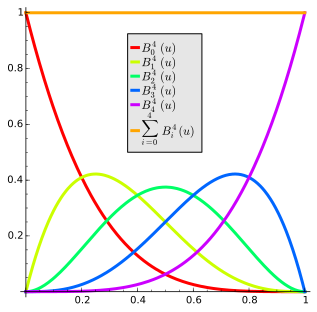
\includegraphics[scale=0.8]{images/Bernstein_Polynomials.png}
\end{figure}

\begin{Bemerkung}
Die Bernsteinpolynome vom Grad $n$ bilden eine Basis des Vektorraums der Polynome vom Grad $n$ im Intervall $[0,1]$.
\end{Bemerkung}

\begin{Satz}
Es gilt die Rekursionsformel
\begin{align*}
B_i^n(t) = (1-t) \cdot B^{n-1}_{i}(t) + t \cdot B^{n-1}_{i-1}(t)
\end{align*}
mit $B^0_0(t) = 1$ und $B^i_n(t) = 0$ für $i<0$ oder $i>n$.
\end{Satz}
\begin{proof}
Folgt fast direkt aus der Rekursionsformel des Binomialkoeffizienten
\begin{align*}
\begin{pmatrix} n \\ i \end{pmatrix} = \begin{pmatrix} n-1 \\ i \end{pmatrix} + \begin{pmatrix} n-1 \\ i-1 \end{pmatrix} 
\end{align*}
 \begin{figure}[H]
\centering
\includegraphics[scale=0.2]{images/pascal.png}
\end{figure}
\end{proof}


\begin{Definition}
Seien $b_0, \hdots b_n \in \mathbb{R}^3$. Dann heißt die Kurve
\begin{align*}
B^n(t) := \sum_{i = 0}^{n} B_i^n(t) \cdot  b_i \; , t \in [0,1] 
\end{align*} 
eine Bezierkurve vom Grad $n$. Die $b_i$ werden auch Kontrollpunkte genannt.
Für ein beliebiges Intervall $[a,b]$ definieren wir
\begin{align*}
B^n_{[a,b]} (t):=  B^n\biggl( \frac{t-a }{a-b} \biggr) \; , t \in [a,b] \; .
\end{align*} 
\end{Definition}


\begin{Satz}
Eine Bezierkurve hat die Ableitung
\begin{itemize}
\item $(B^n)'(t) = n \cdot \sum_{j = 0}^{n-1} B_{j}^{n-1}(t) \cdot (b_{j+1} - b_j) \; ,$ und nach der Kettenregel
\item $(B^n_{[a,b]})'(t) = \frac{1}{b-a} (B^n)' \bigl(\frac{t -a}{b-a} \bigr)$  für ein beliebiges Parameterintervall.
\end{itemize}
\end{Satz}

\begin{Satz}[Algorithmus von de Casteljau]
Sei $B^n(t) := \sum_{i = 0}^{n} B_i^n(t) \cdot  b_i$ eine Bezierkurve. Für ein 
$t_0 \in [0,1]$ definieren wir rekursiv  
\begin{align*}
b_i^k := \begin{cases}
b_i   & i= 0, \hdots,  n \\
(1-t_0) \cdot b_{i-1}^{k-1} + t_0 \cdot b_{i}^{k-1} &  i = 1, \hdots , n \; \;   k = 1, \hdots , i 
\end{cases} 
\end{align*}
was sich schematisch folgendermaßen darstellen lässt: 
\begin{align*}
\xymatrix{
b_0   \ar@{}[r]|-{=}  &  b_0^0 \ar[dr]^{\cdot(1-t_0)}  &  & & & & & &  \\
b_1   \ar@{}[r]|-{=}  &  b_1^0  \ar[r]^{\cdot t_0} \ar[dr]^{\cdot(1-t_0)} &   b_1^1  \ar[dr]^{\cdot(1-t_0)} & & & & & & \\
b_2   \ar@{}[r]|-{=}  \ar@{..}[d] &  b_2^0  \ar[r]^{\cdot t_0}  \ar@{..}[d] &   b_2^1 \ar[r]^{\cdot t_0}  \ar@{..}[d] &  b_2^2   \ar@{..}[dr]& & & & & \\
b_{n-1}   \ar@{}[r]|-{=}  &  b_{n-1}^0   \ar[r]^{\cdot t_0}  \ar[dr]^{\cdot(1-t_0)} &    b_{n-1}^1   \ar[r]^{\cdot t_0}  \ar[dr]^{\cdot(1-t_0)} &  b_{n-1}^2  \ar@{..}[r] &  
b_{n-1}^{n-1}  \ar[dr]^{\cdot(1-t_0)} & & & & \\
b_{n}   \ar@{}[r]|-{=}  &  b_{n}^0  \ar[r]^{\cdot t_0}  &    b_{n}^1   \ar[r]^{\cdot t_0}  &  b_{n}^2  \ar@{..}[r] & b_{n}^{n-1}   \ar[r]^{\cdot t_0}& b_{n}^{n}& & & 
}
\end{align*}
Dann gilt $b_n^n = B^n(t_0)$.
\end{Satz}

\input{deCasteljau.pdf_t} 



\begin{Definition}[Patching]
Seien $B^n(t)$ und $B^m(t)$  Bezierkurven. Man spricht von eimen $C^0$-patching, falls
 \end{Definition}

\input{bezier_patch.pdf_t} 


\begin{figure}[H]
\centering
Ein Rendering der Utah Teekanne, eines der weit verbreitetsten 3D-Modelle in der Computergrafik. Sie wurde mit Bezierflächen modelliert\\
\includegraphics[scale=0.1]{images/Utah_teapot.png}
\end{figure}

\subsubsection{Subdivision}


\subsection{Labor}


\section{Echtzeitvisualisierung und OpenGL}
\subsection{Geschichte}
\subsection{GL-Pipeline}
\subsection{Lokale Beleuchtungsmodelle}
\subsubsection{Ideale Reflexionen und Lichtbrechungen}
\subsubsection{Lambert  Modell}
\subsubsection{Phong Modell}

\subsection{Texturen und UV-Mapping}
\subsection{Shaderprogrammierung und standard Algorithmen}
\subsubsection{Syntax und Funktionsumfang}
\subsubsection{Flat  shading}
\subsubsection{Phong  shading}
\subsubsection{Bumpmapping}
\subsubsection{Displacementmapping}
\subsubsection{Shadowmap}

\subsection{Labor}
\subsubsection{WebGL}





\section{Raytracing}

\subsection{Farbwahrnehmung und Farbmodelle}
\subsection{Globale Beleuchtungsmodelle und Rendergleichung}
\subsection{Raycasting}
\subsubsection{"Klassisches" Raytracing}
\subsubsection{Monte Carlo Integration und Pathtracing}
\subsubsection{Datenstrukturen für Bereichsabfragen}

\subsection{Raymarching}
\subsection{Labor}
\subsubsection{Blender}
\subsubsection{Echtzeitfähiges Raymarching in WebGL}

\section{Animation und Simulation}
\subsection{Keyframe Animation}
\subsection{Partikelsysteme}
\subsection{Elemente der Kollisionserkennung}
\subsection{Labor}

\end{document}
